\chapter{\IfLanguageName{dutch}{Stand van zaken}{State of the art}}
\label{ch:stand-van-zaken}

% Tip: Begin elk hoofdstuk met een paragraaf inleiding die beschrijft hoe
% dit hoofdstuk past binnen het geheel van de bachelorproef. Geef in het
% bijzonder aan wat de link is met het vorige en volgende hoofdstuk.

% Pas na deze inleidende paragraaf komt de eerste sectiehoofding.


\section{Artificiële Intelligentie: Introductie en Termen}
\label{sec:artificiëleintelligentieintroductie}
In een eerste hoofdstuk wordt het begrip artificiële intelligentie besproken. Deze term is heel belangrijk, want het analyseren van reviews is een toepassing hiervan. Ook de geschiedenis wordt hier kort besproken. Daarna wordt machine learning beter uitgelegd. Machine learning is een belangrijk deelveld van artificiële intelligentie. Vervolgens worden deep learning en neurale netwerken besproken. Deze technieken zijn nodig om de reviews te analyseren. 

\subsection{Artificiële Intelligentie}
\label{sec:artificiëleintelligentie}
Een van de hoofdbegrippen van deze bachelorproef is artificiële intelligentie (AI). \gls{AI} is een tak van de wetenschap die zich bezighoudt met het onderzoek naar hoe computers of machines het denkvermogen, leervermogen en keuzeproces van de mens proberen na te bootsen. Het hoofddoel van AI is om naar de vaardigheden van de mens te kunnen handelen. \autocite{IBM2021}

AI is echter niet zo’n vergezocht concept als velen denken. AI bevindt zich overal rondom ons, ook in het dagelijkse leven. Enkele voorbeelden: een chatbot van een website waarop iemand een item wilt bestellen, fotoherkenning of aanbevelingen van ons favoriete streamingplatform. \autocite{IBM2021}

Artificiële intelligentie kan opgedeeld worden in cognitieve intelligentie en emotionele intelligentie. Onder cognitieve intelligentie wordt begrepen dat een AI zijn ervaring gebruikt om toekomstige beslissingen te maken. Bij emotionele intelligentie probeert de AI de mens en zijn emoties echt te begrijpen. \autocite{Andreas2018}

\textcite{Kraaijvanger2012} schreef een artikel over de \gls{TuringTest}. Dit is een begrip dat vaak met artificiële intelligentie geassocieerd wordt. Bij een Turing Test wordt er gekeken of een computer (AI) een persoon kan laten denken dat de computer een mens is. Is dit het geval, dan wordt de computer aanzien als intelligent. Deze Turing Test werd in het leven geroepen in 1950 door Alan Turing. 

\subsection{De geschiedenis van Artificiële Intelligentie}
\label{sec:artificiëleintelligentiegeschiedenis}

Officieel werd er voor het eerst over het onderzoeksgebied artificiële intelligentie gesproken in 1956, op een conferentie in Hanover, New Hampshire. Hier werd de term ‘kunstmatige intelligentie’ voor het eerst in het leven geroepen. Het concept artificiële intelligentie was niet gemakkelijk en de vooruitgang vorderde traag, waardoor in de jaren ‘70 de interesse voor AI snel daalde. Vanaf de jaren ‘80 begon de Britse regering het onderzoek naar AI opnieuw te financieren, waardoor vooruitgang opeens versnelde. \autocite{Anyoha2017}

In het artikel van \textcite{Anyoha2017} wordt nadruk gelegd op het jaar 1997. Dit was een belangrijk jaar voor de wetenschap. Dit was het jaar waarin Deep Blue, een computer van IBM de Russische schaakmeester Garry Kasparov versloeg. AI werd vanaf dan gezien als een ‘hot topic’ en deze overwinning betekende een grote stap vooruit voor artificiële intelligentie. In ditzelfde jaar ontwikkelde Dragon Systems spraakherkenningssoftware die geïmplementeerd kon worden in Windows. 
In 2014 werd de bekende chatbot ‘Eugene Goostman’ gemaakt. Deze chatbot nam deel aan een wedstrijd, waarbij 33\% van de jury de robot als een mens aanzag. Velen zijn daarom van mening dat de chatbot de hierboven besproken Turing Test doorstaan heeft. \autocite{Anyoha2017}
 
Artificiële intelligentie blijft tot op vandaag de dag een veelbesproken onderwerp en vooruitgang op dit gebied gaat aan een razend tempo. 

\subsection{Machine Learning}
\label{sec:machinelearning}
\gls{MachineLearning} is een deelveld van artificiële intelligentie. Het verschil is dat machine learning leert van fouten en successen en zichzelf programmeert om een specifieke taak zo goed mogelijk uit te voeren, met meer precisie. Een voorbeeld hiervan: YouTube beveelt de gebruiker steeds nieuwe video’s aan die hem of haar kunnen interesseren aan de hand van video’s die de gebruiker al eerder heeft bekeken. \autocite{IBM2021}

Als men spreekt over machinaal leren (of machine learning), dan spreekt men over algoritmen. Deze kan men definiëren als “een opeenvolging van statistische verwerkingsstappen”. Bij machinaal leren worden deze algoritmen getraind met het doel om patronen en herkenningspunten te ontdekken in gegevens en op basis van deze gegevens beslissingen of voorspellingen te maken op basis van nieuwe gegevens. \autocite{IBM2020a}

Machines kunnen op een aantal verschillende manieren leren, of een mix van verschillende technieken toepassen. Deze technieken kunnen in 3 categorieën ingedeeld worden:

\subsubsection{Supervised Learning}
\label{sec:supervisedlearning}
Bij \gls{SupervisedLearning} krijgt het algoritme gelabelde gegevens. Bijvoorbeeld bij een dataset van de winkelketen Zalando krijgt elk item een label: ‘kledij’ of ‘schoenen’. Het algoritme leert aan de hand van deze gelabelde gegevens en kan zo toekomstige gegevens in een categorie opdelen. Wanneer de labels reële getallen zijn, gaat het over \textbf{regressie}. Een voorbeeld van regressie is het voorspellen van het gewicht van een persoon aan de hand van zijn of haar lengte. Wanneer de labels voorgedefinieerde klassen voorstellen, dan gaat het over \textbf{classificatie}. Een voorbeeld hiervan is spamdetectie, waarbij de gegevens opgedeeld worden in ‘spam’ en ‘geen spam’.\autocite{Lievens2020} 

\subsubsection{Unsupervised Learning}
\label{sec:unsupervisedlearning}
Bij \gls{UnsupervisedLearning} krijgt het algoritme ongelabelde gegevens. Het doel hiervan is om een ‘structuur’ te ontdekken in de dataset. Clustering is de bekendste taak van unsupervised learning. Hierbij wordt de data in groepen (clusters) opgedeeld. Een voorbeeld hiervan is een website van een krant. Hier worden de verschillende artikels gegroepeerd volgens onderwerp. \autocite{Lievens2020}
Andere taken van unsupervised learning zijn Anomaliedetectie en principale-componentenanalyse. Anomaliedetectie detecteert automatisch gegevens die ver van de standaard liggen. Principale-componentenanalyse of PCA deelt de gegevens op in principale componenten zodat de data relevanter is. 

\subsubsection{Reinforcement Learning}
\label{sec:reinforcementlearning}
Bij \gls{ReinforcementLearning} wordt er geen gebruik gemaakt van datasets. Het algoritme leert van een dynamische omgeving. Deze omgeving geeft een reeks van beloningssignalen. Een negatief signaal betekent een ‘slechte’ handeling van de machine, terwijl een positief signaal een ‘goede’ handeling van de machine betekent. De machine leert welke acties leiden tot de hoogste totale beloning. \autocite{Lievens2020} Een voorbeeld hiervan is zelfrijdende auto’s. Deze worden beloond om op de weg te blijven.
 
\subsection{Deep Learning}
\label{sec:deeplearning}
\gls{DeepLearning} is een ander deelveld van artificiële intelligentie, meer bepaald een deelveld van machine learning. Bij deep learning leert de robot zichzelf een specifieke taak aan, maar zonder interventie van wetenschappers. \autocite{IBM2020} Bij deep learning wordt het proces van gegevens analyseren steeds herhaald zodat de nauwkeurigheid van toekomstige voorspellingen steeds verbetert. Deep Learning wordt tegenwoordig vaak gebruikt, bijvoorbeeld bij digitale assistenten of spraak-gestuurde huizen. \autocite{IBM2020}
Ook het herkennen van gevoelens in recensies gebeurt aan de hand van deep learning. 
Dankzij deep learning, kunnen algoritmes een output geven die veel accurater is dan bij machine learning. Deep learning werkt met algoritmes die gebaseerd zijn op artificiële neurale netwerken en traint zijn model aan de hand van gelabelde data.


\subsection{Neurale Netwerken}
\label{sec:neuralnetworks}

De meeste deep learning modellen maken gebruik van neurale netwerken. Daarom refereren sommigen naar deep learning modellen als ‘deep neural networks’. 
Een \gls{NeuraalNetwerk} is een netwerk dat gebaseerd is op de hersenstructuur. Een neuraal netwerk bestaat uit neuronen, dit is ook zichtbaar op figuur 2.1. Het netwerk heeft verder enkele input neuronen en enkele output neuronen. Tussen deze inputs en outputs zijn er verbindingen, waar gewichten aan toegekend worden. Alle input neuronen samen worden de inputlaag genoemd, terwijl alle output neuronen de outputlaag vormen. Er kunnen hiertussen nog één of meerdere lagen liggen, die de verborgen lagen worden genoemd. De data gaat doorheen dit model, van de inputlaag, door de verborgen lagen, naar de uitvoerlaag. Hoe Natural Language Processing (NLP) deze lagen gebruikt, wordt later in deze bachelorproef besproken. \autocite{Vervoort2017}

\begin{figure}[!ht]
    \includegraphics[width=\textwidth]{neuraalnetwerk.jpg}
    \caption{\label{neuraalnetwerk}Neuraal Netwerk \autocite{KULeuven2019}.}
\end{figure}

De verschillende lagen voeren verschillende transformaties uit op de inputdata. Omdat de data van de invoer naar de uitvoer stroomt, wordt dit een voorwaarts gericht netwerk genoemd. Op de foto zien we dat de invoerlaag 4 neuronen heeft en de uitvoerlaag heeft 3 neuronen. Dit betekent dat er 3 mogelijke uitkomsten zijn. De verborgen lagen kunnen verschillende types lagen zijn. Zo zijn er bijvoorbeeld convolutional layers, dense layers of pooling layers. 

\subsubsection{Convolutional layers}
\label{sec:convolutionallayers}
\gls{ConvolutionalLayer} worden gebruikt om visuele beelden te analyseren. Deze lagen ontvangen als input een afbeelding en geven als output een volledig andere afbeelding. Om dit te kunnen doen bevat een convolutional layer een filter die over de afbeelding geschoven wordt. Fotoherkenning is één van de bekendste voorbeelden waarbij dit soort lagen gebruikt worden. \autocite{Nanculef2020}


\subsubsection{Dense layers}
\label{sec:denselayers}
\gls{DenseLayer} zijn de lagen die het vaakst voorkomen bij deep neural networks. Een ander woord voor dense layers is fully connected layers. Deze naam legt de term mooi uit omdat een dense layer volledig verbonden is met alle neuronen in de vorige laag. \autocite{Balachandran2020}


\subsubsection{Pooling layers}
\label{sec:poolinglayers}
\gls{PoolingLayer} zijn lagen die zich bevinden tussen twee convolutional layers. Pooling layers verminderen de complexiteit van de parameters en verminderen het aantal berekeningen die gedaan moeten worden. \autocite{Nanculef2020}

Op elke verbinding tussen de lagen staan er ‘gewichten’. De transformatie van input naar output wordt zo berekend:
output = activatiefunctie x (som van de gewichten van de input nodes). \autocite{Vervoort2017} Wat een activatiefunctie is wordt later besproken. 

\section{Datasets en gegevensvergaring}
\label{sec:datasetsgegevensvergaring}
In dit tweede hoofdstuk wordt besproken wat een dataset juist is, en hoe deze getraind kan worden. Verder worden enkele termen overlopen zoals een activatiefunctie en over-en underfitting. Deze termen zullen zeker terugkomen in het hoofdstuk Methodologie. 

\subsection{Hoe wordt een dataset getraind?}
\label{sec:hoewordtdatasetgetraind}
In de paragraaf hierboven, werd uitgelegd wat deep learning is. Hierbij wordt een taak steeds herhaald, met als doel om de nauwkeurigheid te verbeteren. Deep learning werkt aan de hand van een dataset. 

Een dataset is een verzameling van data. In deze bachelorproef is de data een aantal reviews. Elke review bevat enkele attributen: de auteur, het product, de tekst uit de review,...

Wat betekent het om een dataset te trainen? Bij deep learning gaat de machine steeds over de dataset en leert hij uit de dataset. De nauwkeurigheid van een toekomstige voorspelling over een review wordt zo steeds beter. 

Maar hoe wordt zo een dataset getraind?
Om dit uit te leggen, dienen eerst drie termen verklaard te worden. Ten eerste is er de \gls{TrainingDataset}. Deze dataset is een verzameling van gegevens die gebruikt wordt om het model te trainen. Het model leert dan van deze gegevens. Om bepaalde parameters af te stellen, de hyperparameters, wordt er een \gls{ValidatieDataset} gebruikt. Deze hyperparameters staan ook bekend als metaparameters en worden gebruikt om overfitting te vermijden. De term overfitting wordt later besproken. De resultaten die voort komen uit de validatie dataset worden gebruikt om onze hyperparameters bij te stellen. Ten slotte is er de \gls{TestDataset}. Deze dataset wordt meestal in het begin van onze training afgesplitst van de originele dataset, en wordt na het trainen op ons model toegepast, om te kijken of onze dataset een goede hypothese kan vormen voor nog onbekende gegevens. Dit levert steeds een nauwkeurigheid op. Hoe hoger deze nauwkeurigheid, hoe beter. \autocite{Shah2017} Om een dataset te trainen, moeten er eerst een paar stappen gebeuren. Deze worden hieronder besproken. 

\subsubsection{Data preparatie}
\label{sec:datapreparatie}
Voordat het model getraind kan worden, moeten de gegevens uit de dataset eens overlopen worden. Het aantal attributen van een dataset kan zo verminderd worden. Data die niet nodig is, of die niet van belang is om het model te trainen kunnen alvast verwijderd worden uit de gegevens. 

\subsubsection{Data Cleaning}
\label{sec:datacleaning}
In deze fase van het proces wordt de data ‘opgeschoond’. Soms kan data inconsistent zijn of kunnen er enkele velden missen. Daarom is het interessant om alle rijen te verwijderen die data van het type ‘null’ bevatten. Dit zijn de lege velden van de dataset. Verder is het ook belangrijk om alle niet-numerieke data om te zetten naar numerieke data. Zo kan bijvoorbeeld ‘geslacht’ omgezet worden in 0 en 1 via \gls{OneHotEncoding}. Hierdoor wordt het veldje ‘geslacht’ omgezet in 2 nieuwe velden geslacht\_vrouw en geslacht\_man, waarbij er een 1 toegekend wordt als dit waar is, en een 0 als dit niet waar is. 

\subsubsection{Opzetten van training dataset en test dataset}
\label{sec:opzetten}
Eenmaal de dataset opgekuist en klaargezet is, kan de dataset opgesplitst worden. De dataset wordt opgesplitst in een training set en een test set. Dit gebeurt steeds volgens een ratio. Meestal wordt 70\% van de dataset omgezet naar de training set en 30\% naar de test set. De training dataset wordt gebruikt om het model te trainen, de test dataset wordt gebruikt om te testen of de data wel goed getraind is. 

\subsubsection{Het juiste model kiezen}
\label{sec:model}
Eenmaal de dataset opgesplitst is in een training en een test dataset, is het tijd om het model te kiezen. Voor het onderwerp van deze bachelorproef hebben we een neuraal netwerk nodig. 

Ten eerste is het belangrijk om de juiste lagen te kiezen om het model te trainen. Eerder in deze bachelorproef werden dense layers, pooling layers en convolutional layers besproken. Elke laag heeft zijn voor-en nadelen. 

Ten tweede moet het aantal epochs gekozen worden. Een \gls{Epoch} stelt een volledige cyclus door het neurale netwerk voor. Als het aantal epochs 20 is, zal er 20 keer door het netwerk gegaan worden. Elke keer dat er door het netwerk gegaan wordt, wordt de data opnieuw geanalyseerd en wordt de AI een beetje slimmer en nauwkeuriger.

Eenmaal het model gekozen en getraind is, is het mogelijk om de nauwkeurigheid van het model te berekenen en verder onderzoek te doen. 

\subsection{Overfitting en underfitting}
\label{sec:overunderfitting}

Wanneer er een model getraind wordt, kan het natuurlijk voorvallen dat het model té goed of té slecht getraind is. Hiervoor worden de termen \gls{Overfitting} en \gls{Underfitting} gebruikt. Het model dat getraind wordt moet goed zijn. Een model kan ‘goed’ genoemd worden als het voor toekomstige informatie een goede predictie kan maken. Een model dat de data van de dataset te goed generaliseert, wordt \textbf{overfitting} genoemd. De nauwkeurigheid voor de getrainde data is zeer goed, maar dit is niet het geval voor toekomstige data. Om het anders te zeggen, het model heeft té veel van de training dataset geleerd. Bij \textbf{underfitting} is dit omgekeerd. Het model heeft te weinig van de training dataset geleerd, waardoor predicties met nieuwe data slecht zullen zijn. Bij het trainen van een model, is het belangrijk om een juiste balans te vinden. \autocite{AlMasri2019}

Hoe wordt deze balans gevonden? Hoe worden overfitting en underfitting opgelost? 
Voor \textbf{overfitting} kunnen er enkele technieken toegepast worden om dit te vermijden. 

Overfitting kan herkend worden doordat de training set betere resultaten verkrijgt dan de test dataset. Om overfitting op te lossen kan er ten eerste extra data aan de training dataset toegevoegd worden. Het model kan meer leren als er meer data toegevoegd wordt. Zo is er ook extra diversiteit in de gegevens. Ten tweede kan de complexiteit van het model verminderd worden. Er kan bijvoorbeeld een verborgen laag weggehaald worden, of het aantal neuronen in de lagen kan verminderd worden. Ten derde kan er cross-validatie toegepast worden. Er worden kleine mini train-test datasets gemaakt om het model te verfijnen. Er zijn natuurlijk nog andere methoden om overfitting te vermijden. \autocite{Datascience2021}

Omgekeerd, moet er ook rekening worden gehouden met underfitting. Om underfitting te vermijden kan ten eerste de complexiteit van het model verhoogd worden. Ten tweede kan het aantal features verhoogd worden en kan onnodige data uit de dataset verwijderd worden. Ten slotte kan ook het aantal epochs (cyclus die door de volledige dataset gaat) verhoogd worden zodat het trainen langer duurt en het model betere resultaten geeft. \autocite{GeeksforGeeks2020}

\subsection{Activatiefunctie van een neuraal netwerk}
\label{sec:activatiefunctie}

De \gls{ActivatieFunctie} van een neuraal netwerk is een functie die de inputdata van een neuron transformeert in output. Er bestaan meerdere activatiefuncties, de juiste activatiefunctie voor het netwerk kiezen heeft een grote impact op het netwerk. De verborgen lagen gebruiken meestal dezelfde activatiefunctie, maar dit kan een andere activatiefunctie zijn dan die van de outputlaag. Alle afbeeldingen van de activatiefuncties zijn gebaseerd op informatie gevonden uit het artikel van \textcite{Brownlee2021}. 

\subsubsection{ReLU}
\label{sec:ReLU}

De eerste mogelijke activatiefunctie is de \gls{ReLU} (of rectified linear activatiefunctie). De ReLU is, zoals de naam al aangeeft, een lineaire functie. Wanneer de output positief is, zal de ReLU gewoon de output nemen. Als de output negatief is zal de ReLU daar een waarde van 0 aan toekennen. Dit betekent dus dat op de ReLU grafiek, de functie nooit negatief zal zijn. De ReLU wordt het vaakste gebruikt bij verborgen lagen. \autocite{Brownlee2021}

\begin{figure}[!htbp]
    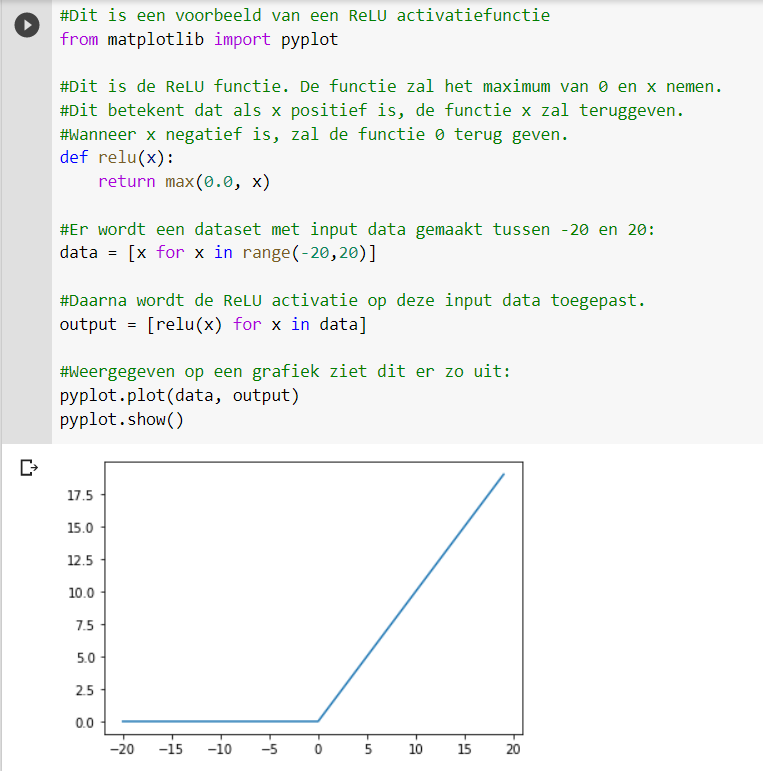
\includegraphics[width=\textwidth]{ReLU.PNG}
    \caption{\label{ReLU}De ReLU activatiefunctie \autocite{Brownlee2021}.}
\end{figure}
\FloatBarrier


\subsubsection{Sigmoïde}
\label{sec:sigmoide}

De \gls{Sigmoïde} activatiefunctie zorgt ervoor dat elke input een output tussen 0 en 1 wordt. Ook hier kan de grafiek dus nooit in het negatieve gaan. Hoe hoger de input, hoe dichter bij 1 en omgekeerd. De sigmoïde functie wordt ook gebruikt bij logistische regressie, maar dit wordt niet in deze bachelorproef besproken. \autocite{Brownlee2021} De sigmoïde activatiefunctie gebeurt als volgt:

\begin{figure}[!htbp]
    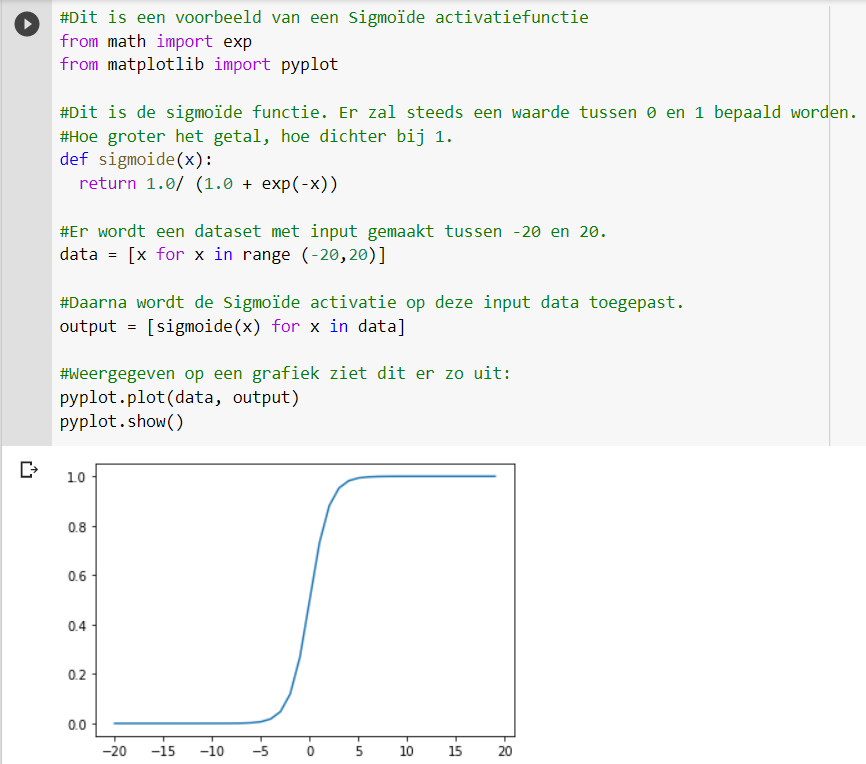
\includegraphics[width=\textwidth]{sigmoide.PNG}
    \caption{\label{sigmoide}De sigmoïde activatiefunctie \autocite{Brownlee2021}.}
\end{figure}
\FloatBarrier


\subsubsection{Tanh}
\label{sec:tanh}

De \gls{Tanh} activatiefunctie lijkt een beetje op de sigmoïde activatiefunctie in die zin dat ze allebei die S-vorm vertonen. Het verschil tussen de sigmoïde activatiefunctie en de tanh activatiefunctie is dat de tanh activatiefunctie de input omzet in waarden tussen -1 en 1. Waardoor dit de enige activatiefunctie is waarbij de output negatief kan zijn. Hoe groter de input, hoe dichter bij 1, hoe kleiner de input, hoe dichter bij -1. \autocite{Brownlee2021}

\begin{figure}[!htbp]
    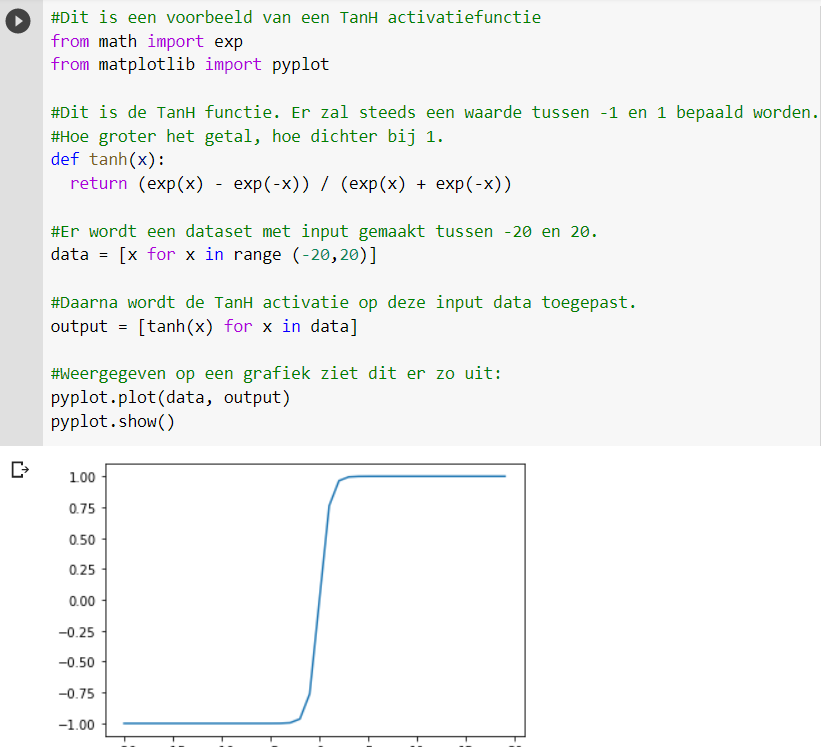
\includegraphics[width=\textwidth]{tanh.PNG}
    \caption{\label{tanh}De Tanh activatiefunctie \autocite{Brownlee2021}.}
\end{figure}
\FloatBarrier


\section{Natural Language Processing}
\label{sec:NLP}

In dit hoofdstuk wordt besproken wat NLP of Natural Language Processing juist is. Daarnaast worden enkele interessante technieken besproken die in het onderzoek naar NLP zeker toegepast zullen worden. 

\subsection{Wat is NLP?}
\label{sec:WatisNLP}
NLP staat voor \gls{NLP} en is het hoofdonderwerp van deze bachelorproef. Natural Language processing is het deelveld van artificiële intelligentie dat zich bezighoudt met taal. Deze term geeft machines of computers de mogelijkheid om tekst of spraak te herkennen. NLP maakt gebruik van machine learning en deep learning om taal te herkennen. Deze onderwerpen werden hiervoor al besproken. De NLP technologie stelt een machine niet enkel in staat om tekst te herkennen, maar ook om deze te ‘begrijpen’. Zo zijn de vertaaltools begonnen. NLP houdt niet enkel het herkennen van teksten in, maar ook het vertalen en begrijpen van teksten. Enkele voorbeelden hiervan zijn Google Translate en DeepL. NLP komt niet enkel voor in vertaaltools, maar ook bij digitale assistenten of chatbots. \autocite{IBM2020}

Het analyseren van teksten, zinnen of uitgesproken woorden is niet gemakkelijk. De menselijke taal is heel complex. Mensen drukken zich vaak op heel veel verschillende manieren uit, en het is aan de machine om dit te interpreteren. Naast honderden talen, heeft elke taal nog vele dialecten. Daarnaast heeft elke taal zijn eigen grammaticaregels, termen en syntaxisregels.
Op vlak van spraak gestuurde NLP, verspreekt een persoon zich al snel, of kan deze met een dialect praten. \autocite{sas2020}

Natural Language Processing heeft veel technieken om de menselijke taal te interpreteren. NLP breekt de volledige teksten op in stukjes. Daarna probeert NLP de relaties tussen deze stukjes te analyseren en begrijpen. Enkele belangrijke taken van NLP zijn tokenization and parsing, language detection en lemmatization/stemming. \autocite{sas2020}

\subsubsection{Language detection}
\label{sec:Languagedetection}

Wanneer een tekst onderzocht wordt, moet de machine eerst bepalen in welke taal deze tekst staat. Wanneer er meerdere talen in 1 tekst staan, worden er meerdere classificatie modellen gemaakt, 1 per taal. In figuur 2.5 wordt dit getest met de zin ‘vandaag is een prachtige dag' in verschillende talen. 

\begin{figure}[!htbp]
    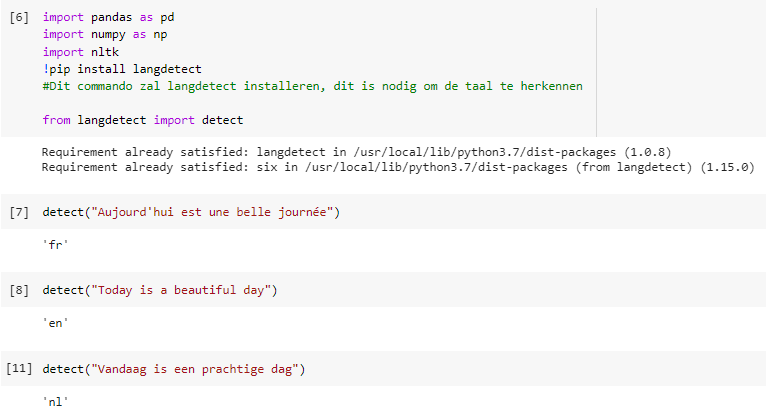
\includegraphics[width=\textwidth]{langdetect.PNG}
    \caption{\label{languagedetection}Language Detection \autocite{sas2020}.}
\end{figure}
\FloatBarrier

\subsubsection{Tokenization and parsing}
\label{sec:Tokenization}

Tokenization is een NLP techniek waarbij een string of zin in kleinere tokens opgedeeld wordt. Tokenization is belangrijk omdat in NLP de tekst geanalyseerd wordt op tokens. 

\begin{figure}[!htbp]
    \includegraphics[width=\textwidth]{tokenization.PNG}
    \caption{\label{tokenization}Tokenization and parsing \autocite{sas2020}.}
\end{figure}
\FloatBarrier

\subsubsection{Stemming and lemmatization}
\label{sec:stemming}

Stemming en lemmatization zijn twee NLP technieken die lijken op elkaar, maar toch verschillen op bepaalde vlakken. Het zijn beiden tekst normalisatie technieken. Stemming en lemmatization baseren zich allebei op het feit dat woorden afgestamd zijn van een ander woord. Zo hebben we bijvoorbeeld het werkwoord ‘spelen’. Van het werkwoord spelen kan gezegd worden dat het afstamt van speel. ‘Speelt’ en ‘speelde’ stammen ook af van de stam ‘speel’. Het verschil tussen stemming en lemmatization is dat lemmatization rekening houdt met de context van het woord. \autocite{sas2020}

\begin{figure}[!htbp]
    \includegraphics[width=\textwidth]{stemming.png}
    \caption{\label{stemming}Stemming and lemmatization \autocite{sas2020}.}
\end{figure}
\FloatBarrier

NLP wordt vaak gebruikt in het alledaagse leven. Alexa en Siri zijn heel gekende voorbeelden, maar deze techniek wordt ook in veel andere toepassingen gebruikt, zoals bij spam filtering. 

\subsection{Text Analytics}
\label{sec:textanalytics}

\gls{TextAnalytics} of text mining is een techniek die veel wordt teruggevonden in Natural Language Processing. Dankzij deze techniek wordt tekst zonder structuur gemakkelijk omgezet in een gestructureerde dataset. \autocite{Linguamatics2021} Deze dataset is nodig om het model te kunnen trainen, zoals uitgelegd in Hoofdstuk 2: Datasets en gegevensvergaring.
Text mining is enorm belangrijk. In het dagelijkse leven komt iedereen in aanraking met tekst, denk maar aan e-mails, digitale assistenten, chatbots of posten op sociale media. In deze bachelorproef worden volzinnen uit recensies geanalyseerd op een positieve of negatieve connotatie. Text mining zal hier aan te pas komen op deze ongestructureerde volzinnen in een gestructureerde dataset om te vormen. Tijdens dit proces zal NLP aan de hand van machine learning toegepast worden. 

\section{Sentiment Analysis}
\label{sec:sentimentanalysis}

In dit hoofdstuk wordt het begrip Sentiment Analysis besproken. Ten tweede wordt ook kort ingegaan op wat gevoelswaarden juist zijn. Verder wordt ook de problematiek van deze bachelorproef uitgelegd: waarom is het nu zo moeilijk om sentiment uit een tekst te halen?  

\subsection{Wat is Sentiment Analysis?}
\label{sec:watissentimentanalysis}

\gls{SentimentAnalysis} is het onderzoek dat in deze bachelorproef wordt gevoerd. Er wordt een sentiment analyse uitgevoerd op recensies. Sentiment analyse is een Natural Language Processing (NLP) techniek die gebruikt wordt om te onderzoeken of een tekst een positieve, neutrale of negatieve connotatie heeft. Klanten drukken vaak hun gevoelens uit in de vorm van recensies. Het is voor bedrijven essentieel om op deze gevoelens in te spelen. Met sentiment analysis kan een bedrijf de feedback van de klant analyseren en begrijpen. \autocite{MonkeyLearn2021}
 
Dankzij Sentiment Analysis kan een bedrijf te weten komen wat er in het hoofd van hun klanten omgaat. Sentiment Analysis kan niet enkel de reviews van de klant analyseren als positief/negatief, maar kan dit ook koppelen aan een bepaald product. Zo weet het bedrijf van welk product de klanten het meest tevreden zijn. \autocite{MonkeyLearn2021}

Er zijn verschillende soorten sentiment analysis, zoals emotiedetectie, multilingual sentiment analysis en aspect-based sentiment analysis. 

Emotiedetectie is een soort sentiment analysis die zich bezig houdt met het achterhalen van gevoelens uit teksten. Deze gevoelens kunnen boosheid, blijheid, verdriet en veel meer uitdrukken. \autocite{MonkeyLearn2021}

Aspect-based sentiment analysis is de techniek die toegepast zal worden in het onderzoek van deze bachelorproef. Bij deze techniek komt een bedrijf te weten over welke features of producten de klant zich positief of negatief uitdrukt. \autocite{MonkeyLearn2021}

Aspect-based sentiment analysis analyseert ten eerste de sentimenten van de tekst, en ten tweede ook de aspecten (features of producten) waarover de gevoelens gaan.
 
Multilingual sentiment analysis is hetzelfde als sentiment analysis, maar met de gedachte dat een review in de eigen taal moet geanalyseerd worden, om geen context of connotatie te verliezen. \autocite{MonkeyLearn2021}

\subsection{Sentiment Analysis en Algoritmen}
\label{sec:sentimentanalysisenalgoritmen}

Bij het implementeren van het sentiment analysis model, zijn er drie soorten algoritmes die men kan gebruiken. (MonkeyLearn, 2021)

\subsubsection{Rule based}
\label{rule based}

Rule based algoritmen voeren de analyse uit op basis van een set regels. Deze regels kunnen ook bestaan uit NLP technieken zoals tokenization. Algoritmen gebaseerd op regels bepalen twee lijsten. Een lijst met positieve woorden zoals ‘goed’, ‘mooi’, ‘prachtig’ en ‘super’, en een lijst met negatieve woorden zoals ‘slecht’, ‘ontevreden’,  en  ‘lelijk’. Daarna telt het algoritme het aantal woorden uit deze lijst dat voorkomt in de gegeven tekst of review. Als er meer positieve woorden geteld zijn dan negatieve, dan wordt de tekst gezien als positief. Dit is dus omgekeerd ook het geval. \autocite{MonkeyLearn2021}

\subsubsection{Automatic}
\label{automatic}

Bij dit algoritme gebruikt men machine learning technieken, waarbij de data getraind wordt. Wanneer we dan een tekst of review in dit algoritme steken, zal het algoritme daar een negatieve, neutrale of positieve connotatie aan toekennen. Dit gebeurt aan de hand van deep learning. \autocite{MonkeyLearn2021}

\subsubsection{Hybrid}
\label{hybrid}

Bij hybrid algoritmen, maakt het algoritme gebruik van zowel rule-based als automatic algoritmen. \autocite{MonkeyLearn2021}

\subsection{Wat zijn gevoelswaarden?}
\label{gevoelswaarden}

In de context van deze bachelorproef kunnen recensies gevoelswaarden bevatten. Ten eerste zijn er positieve gevoelswaarden. Dit gaat over recensies die lovende kritiek geven over het product of het product aanraden. Enkele voorbeelden van positieve recensies: 

\begin{itemize}
    \item “Ik gebruik de laptop veel onderweg in de trein. Super makkelijk om mee te nemen. Hij start snel op en is perfect voor mijn werk.”
    \item “Zoals altijd super een superspannend boek van een geweldige schrijver. Heerlijk!”
\end{itemize}

Echter kunnen recensies ook negatief zijn. Enkele voorbeelden van negatieve recensies:

\begin{itemize}
    \item “Deze jas heeft geen ritssluiting, waardoor de kans bestaat dat er regen doorkomt. Dit is niet wat ik verwacht had.”
    \item “Teleurstellend. Het telefoonhoesje was beschadigd bij ontvangst.”
\end{itemize}

\subsection{Waarom is het moeilijk voor AI's om sentiment te analyseren?}
\label{moeilijksentimentanalyseren}

\subsubsection{Subjectiviteit}
\label{subjectiviteit}

Gevoelens zijn subjectief. Er zijn talloze manieren waarop iemand zich kan uitdrukken, de één al positiever dan de ander. 

\subsubsection{Context}
\label{context}

De context van bepaalde woorden is ook enorm belangrijk. Een voorbeeld: “De auto was bij aankoop goed beschadigd”. In deze zin zit het woordje ‘goed’, maar dit betekent niet dat de review een positieve connotatie heeft, integendeel. \autocite{MonkeyLearn2021}

\subsubsection{Ironie en sarcasme}
\label{ironiesarcasme}

Ironie en sarcasme zijn twee zaken die een machine moeilijk kan herkennen. Wanneer iemand ironie of sarcasme gebruikt, drukt hij zijn negatieve gevoelens over een bepaald aspect uit met positieve woorden. \autocite{MonkeyLearn2021} Een voorbeeld hiervan: “Wauw, dat ging goed!”. Deze zin kan zowel in een positieve context gezien worden, maar kan ook sarcastisch opgenomen worden. 

\subsubsection{Vergelijkingen}
\label{vergelijkingen}

Ook vergelijkingen kunnen door elkaar gebruikt worden. We kunnen ‘beter dan’ gebruiken in verschillende contexten. 

\begin{itemize}
    \item “Deze smartphone is beter dan de vorige versie.”
\end{itemize}

Deze review heeft duidelijk een positieve context, maar we kunnen ook deze review analyseren:


\begin{itemize}
    \item “Deze smartphone is trager dan gewoonlijk, maar het is beter dan niets.”
\end{itemize}

In deze context, is ‘beter dan’ helemaal niet positief. Dit toont ook aan waarom het voor artificiële intelligentie zo moeilijk is om een sentiment uit een zin te halen. 


\section{Gevoelswaarden detecteren in teksten}
\label{gevoelswaardendetecteren}

Sentiment of gevoelswaarden kunnen op verschillende manieren gedetecteerd worden in teksten. Daarom worden in dit hoofdstuk enkele manieren besproken die in de methodologie zullen toegepast worden. 

\subsection{SaaS (Software as a Service)}
\label{saas}

Wanneer een model voor sentiment analysis zou geschreven moeten worden, dan zou er een team aan programmeurs en een grote som geld nodig zijn. Daarom is het interessant om SaaS-tools te gebruiken. SaaS platforms bieden software als een service aan. Dit betekent dat de gebruiker deze software via het internet kan gebruiken, maar deze niet op zijn computer kan downloaden. \autocite{Marketing2021} Deze techniek wordt zeker gebruikt in het methodologie-gedeelte. De software-platforms hieronder zijn voorbeelden van \gls{SAAS}. 

\subsubsection{MonkeyLearn}
\label{monkeylearn}

Monkeylearn is een platform dat services aanbiedt om tekst te analyseren aan de hand van machine learning en sentiment analysis. Het voorziet een grafische user interface om zelf reviews in te geven en deze te trainen. \autocite{Maguire2021} Het platform van MonkeyLearn zal getest en gebruikt worden tijdens het onderzoek.

\subsubsection{Text Analytics API}
\label{textanalytics}

Text Analytics API is een service die NLP aan de gebruiker aanbiedt. Technieken zoals sentiment analysis en opinion mining kunnen worden uitgevoerd aan de hand van deze service. Deze API maakt deel uit van Azure Cognitive Services. \autocite{Microsoft2020} Deze Tekst Analytics API kan gebruikt worden in Visual Studio Code aan de hand van REST API. Ook deze service zal getest en gebruikt worden tijdens het onderzoek.

Naast SaaS-tools, kan men ook zelf een dataset zoeken en deze trainen. Dit wordt verder besproken in het volgende hoofdstuk.

\section{De Datasets}
\label{datasets} 

Zoals hiervoor aangehaald, is het natuurlijk ook mogelijk om zelf een dataset te gebruiken en deze te trainen. In dit onderzoek worden er twee datasets gebruikt.

\subsection{Amazon Dataset}
\label{amazon}

De eerste dataset is de \textbf{Amazon dataset}. Deze dataset bevat reviews van de producten die op de populaire website Amazon verkocht worden. Deze dataset bevat meer dan 233 miljoen reviews, daardoor zal niet deze volledige dataset gebruikt worden. De reviews van deze dataset werden verzameld tussen 1996 en 2018. \autocite{Ni2019} Een voorbeeld van hoe 1 review er uit ziet in de dataset kan hieronder gevonden worden: 
  
\begin{table}[]
    \begin{tabular}{@{}|l|l|@{}}
        \toprule
        \textbf{Attribute} & \textbf{Content}                                                                                                                                                                                                                                                                                        \\ \midrule
        reviewerID         & A2SUAM1J3GNN3B                                                                                                                                                                                                                                                                                          \\
        asin               & 0000013714                                                                                                                                                                                                                                                                                              \\
        reviewerName       & J. McDonald                                                                                                                                                                                                                                                                                             \\
        helpful            & {[}2,3{]}                                                                                                                                                                                                                                                                                               \\
        reviewText         & \begin{tabular}[c]{@{}l@{}}I bought this for my husband who plays the piano. \\ He is having a wonderful time playing these old hymns. \\ The music is at times hard to read because we think the book\\  was published for singing from more than playing from. \\ Great purchase though!\end{tabular} \\
        overall            & 5.0                                                                                                                                                                                                                                                                                                     \\
        summary            & Heavenly Highway Hymns                                                                                                                                                                                                                                                                                  \\
        unixReviewTime     & 1251800000                                                                                                                                                                                                                                                                                              \\
        reviewTime         & 09 13, 2009                                                                                                                                                                                                                                                                                             \\ \bottomrule
    \end{tabular}
    \caption{Attributen van de Amazon Dataset}
    \label{tab:amazondataset}
\end{table}

\subsection{Twitter US Airline Sentiment Dataset}
\label{twitter}

De tweede dataset is de \textbf{Twitter US Airline Sentiment dataset}. Deze dataset bevat reviews in de vorm van tweets. Deze reviews gaan over de bekendste US vluchtmaatschappijen.\autocite{Kaggle2020} Een voorbeeld van hoe 1 review er uit ziet in de database kan hieronder gevonden worden:
\begin{table}[]
    \begin{tabular}{@{}|l|l|@{}}
        \toprule
        \textbf{Attribute}             & \textbf{Content}            \\ \midrule
        tweet\_id                      & 570306133677760513          \\
        airline\_sentiment             & neutral                     \\
        airline\_sentiment\_confidence & 0.3486                      \\
        negativereason                 & Bad Flight                  \\
        negativereason\_confidence     & 0.7033                      \\
        airline                        & Virgin America              \\
        airline\_sentiment\_gold       & NaN                         \\
        name                           & jnardino                    \\
        negativereason\_gold           & NaN                         \\
        retweet\_count                 & 0                           \\
        text                           & @VirginAmerica, Thanks!     \\
        tweet\_coord                   & NaN                         \\
        tweet\_created                 & 2015-02-24 11:35:52-0800    \\
        tweet\_location                & San Francisco CA            \\
        user\_timezone                 & Pacific Time (US \& Canada) \\ \bottomrule
    \end{tabular}
    \caption{Attributen van de Twitter US Airline Sentiment Dataset}
    \label{tab:twitterdataset}
\end{table}

